\documentclass[UTF8]{ctexart}
\usepackage{geometry}
\usepackage{amsmath}
\usepackage{graphicx} %插入图片的宏包
\usepackage{float} %设置图片浮动位置的宏包
\geometry{a4paper,scale=0.8}
\sectionfont{\bfseries\Large\raggedright}

\title{deep-learning笔记}
\author{徐世桐}
\date{}
\begin{document}
\maketitle

\section{基本定义}
\noindent \textbf{label标签}:输出结果,$\hat{y} $为计算得到的结果,$y$为实际测量结果\\
\textbf{feature特征}:用于预测标签的输入变量,$x^{(i)}_j$为第i组sample第j号特征\\
\textbf{sample样本}:一组特征的取值和对应的标签输出,样本编号集合称$B$\\
\textbf{hyperparameter超参数}:人为设定的参数。如样本个数(批量大小batch size)$|B|$,学习率$\eta $。少数情况下通过学习得到\\
\textbf{全连接层fully-connected layer/稠密层dense layer}:此层所有节点都分别和前一层所有节点连接
\textbf{softmax函数}:$softmax(Y) = \frac{exp(y)}{\sum_{y' \in Y} exp(y') } $,将数值输出转化为概率值,1. 值为正 2. 值总和为1
\textbf{cross entropy交叉熵}

  定义:分部p 和 分部q 间的 cross entropy $H(p, q) = -E_p(\log (q))$。为 expected value of $log (q)$ with respect to distribution p

  公式:$H(y^{(i)}, \hat{y}^{(i)}) = -\sum_{j\in B}y^{(i)}log(\hat{y}^{(i)})$

  使用:联系两个值概率分部间的差异,即可将数值输出$\hat{y}$和分类结果$y$直接做对比,无需softmax


\section{linear regression线性回归}
\noindent \textbf{平方代价函数}:$J(\theta ) = \frac{1}{n} \sum_{i = 1}^{n} J^{(i)}(\theta )$,为所有样本误差的平均值\\
\textbf{迭代}:$\theta_i = \theta_i - \frac{\eta}{|B|}\sum_{i\in B} \frac{d J^{(i)}(\theta)}{d \theta_i}$,即对所有sample训练一次,得到label差值,对每一参数减 斜率*学习率 的平均值
  
  当使用平方代价函数:
  
  \quad $\theta_i = \theta_i - \frac{\eta}{|B|}\sum_{i\in B} x^{(j)}_i(x^{(j)}_1\theta_1 + x^{(j)}_2\theta_2 + ... + const - y^{(j)}) = \theta_i - \frac{\eta}{|B|}\sum_{i\in B}x^{(i)}(\hat{y}^{(j)} - y^{(j)})$

  \quad $const = const - \frac{\eta}{|B|}\sum_{i\in B} (x^{(j)}_1\theta_1 + x^{(j)}_2\theta_2 + ... + const - y^{(i)}) = const - \frac{\eta}{|B|}\sum_{i\in B}(\hat{y}^{(j)} - y^{(j)})$

  \quad 对样本i的偏导数向量为$\nabla _{\theta}J^{(i)}(\theta) = 
    \begin{bmatrix}
    x^{(i)}_1 \\
    x^{(i)}_2 \\
    ... \\
    1
    \end{bmatrix}(\hat{y}^{(i)} - y^{(i)})
    $\\
\textbf{交叉熵代价函数}:$J(\theta) = \frac{1}{|B|}\sum_{i\in B} H(y^{(i)}, \hat{y}^{(i)})$\\
\textbf{softmax线性回归}:单层神经网络,使用softmax代价函数\\
\textbf{过拟合问题}

  \textbf{1.权重衰减}:在代价函数中惩罚高权重的值,尽可能使所有权重值减小

  \quad 新代价函数 = $J(\theta) + \frac{\lambda}{2}\sum_{w\in W}w^2$,即 $J(\theta) + \frac{\lambda}{2} * $ 所有权重的平方和。$\lambda$为超参数,决定权重衰减的程度

  \textbf{2.丢弃法}

  \quad 每一权重(不包括const)有p的几率 $\theta' = 0$,有1-p的几率 $\theta' = \frac{\theta}{1-p}$

  \quad 为了得到确切的值,在测试模型时较少使用\\
\textbf{初始化参数}

  \textbf{1.MXNet默认随机初始化}:所有权重$\sim N(0, 1)$的normal distribution,所有const取0

  \textbf{2.Xavier随机初始化}:对一全连接层,输入个数a,输出个数b,则所有参数$\sim U(-\sqrt{\frac{6}{a+b}}, \sqrt{\frac{6}{a+b}})$\\
\textbf{预处理数据集}

  \textbf{1.特征标准化}:$x' = \frac{x - \mu}{\sigma}$,即统计中z值

  \textbf{2.离散值转换成指示特征}:对于一个可取值为A, B, C的离散输入值,转换成3个数值输入。即如果原输入为A,转换后3个数值输入为1,0,0。原离散值为B则转换后为0,1,0


\section{convolutional neural network卷积神经网络}
\noindent \textbf{互相关运算}:

  输入一个二维数组,和\textbf{二维核kernel}进行互相关运算,得到二维数组

  \textbf{二维核/卷积核/filter 过滤器}:在输入数组上滑动,每次和二维数组矩阵一部分按元素相乘,相乘结果求和作为输出矩阵的元素\\
\textbf{二维卷积层}:

  将输入和卷积核做互相关运算,结果加上const作为输出
\section{Deep Feedforward Network (Deep Learning 第6章笔记)}
\noindent \textbf{SVM支持向量机}

  仍通过$w^Tx+b$得到输出,输出仅表示identity,正值说明有identity,负值说明没有

  依据:一个平面的公式为$\beta_0+\beta_1x_1+\beta_2x_2=0$,则当计算$w^Tx+b$得到值后,>0则为平面上方的数据点,<0为下方数据点\\
\textbf{kernel trick}

  kernel method将数据集表示成相近的两个数据点一组的集合$(x_i, x_j)$,kernel method将一对数据变为单一数据点$x=k(x_i, x_j)=\langle \phi (x_i), \phi (x_j)\rangle $

  kernel method使用$\phi $转换数据的纬度,而点乘 化简后无需先计算$\phi (x_i), \phi (x_j)$即可得到新数据点$x$\\
\textbf{manifold hypothesis:}

  当训练数据集合包含大量无规律的数据,则将其中大部分视为无效数据,并只关心落在一个manifold上的数据。

  例:生成图像 文字 声音时数据大多很集中,当像素文字随机分布时生成图像大多无意义\\
\textbf{deep feedforward network/feedforward neural network/multilayer perceptrons MLP:}

  找到$\theta$使得$f(x; \theta )$ 最接近数据y值。$f^*$为最理想的f,即$f^*(x) = y$。$\theta $可为多个参数,如$f(x; w, b) = x^Tw+b$

  $f^*(x) = f^{(3)}(f^{(2)}(f^{(1)}(x)))$,$f^{(1)}$为network第一层。每一$f^{(i)}(x) = \phi (x; \theta )^Tw$

  \textbf{神经网络}

  \quad 1. 结构:

  \quad \quad 输入层没有weight,第一hidden layer得到所有输入层的值。

  \quad \quad hidden layer和输出层所有输出都为0/1,非连续的值

  \quad 2. 一层hidden layer计算方法:$ f^{(i)}(x; W, c) = \sigma (W^Tx + c)$

  \quad \quad x 为前一层的输出向量,输入层x即为训练参数向量。 

  \quad \quad c 为此层常数向量

  \quad \quad z = $W^Tx$为一层hidden layer对输入取得的中间值向量,称logit。a = $\sigma (z + c)$为对z + c每一元素取$\sigma $的结果向量,a即此层的输出。

  \quad \quad W 为此层参数矩阵,行数 = 前层节点数,列数 = 当前层节点数

  \quad \quad X 为多个参数点的训练集中前一层的输出矩阵,行数为数据点个数,列数为前一层节点数

  \quad \quad $XW$ 当W对参数集矩阵操作时,每行向量$z_{i}^T$此时为一层hidden layer各节点对第i参数点的中间值向量。对每行+$c^T$并分别取$\sigma $得到输出矩阵,$a_{ij}$为当使用第i个参数点时此层第j节点的输出

  \textbf{cross entropy}

  \quad 分部p 和 分部q 间的 cross entropy $H(p, q) = -E_p(\log (q))$。为 expected value of $log (q)$ with respect to distribution p

  \textbf{cost function}

  \quad 当使用maximum likelihood估计参数时,cost function$J(\theta )$为 训练输入参数的分部 和 训练结果参数的分部 间cross-entropy: $J(\theta ) = -E_{x, y\sim training\_dataset}(log (p_{model}(y | x)))$

  \quad \quad 对于每一在训练集内的(x, y),求$log (p_{model}(y | x))$, 并求expected value。$p_{model}(y | x)$ 即训练得到的y关于x的分部

  \quad \quad 例:当model为$y = N(f(x; \theta), 1)$正则分部时,$J(\theta) = -E_{x, y\sim data}(y - f(x;\theta))^2 + const$

  \textbf{output layer}

  \quad 当输出层的结果和不为1时,代表数据没有被准确分到某一类中,使用exponentiation and normalisation

  \quad \quad normalisation后结果 $p = \frac{\tilde{p} }{\sum \tilde{p'} } $,为$\tilde{p} $在所有结果中占的比例。$\tilde{p} $为未normalise 值

  \quad 假设输出层结果$\tilde{P} (y | x)$ 有 $log(\tilde{P} (y | x)) = yz$

  \quad \quad $\tilde{P} (y | x) = exp(yz)$

  \quad \quad $P (y | x) = \frac{exp(yz)}{\sum_{y' = 0}^{1} y'z } $,称\textbf{softmax function}

  \quad \quad $P (y | x) = \sigma ((2y - 1)z)$,y,y'为训练目标结果,所以$\sum_{y' = 0}^{1} $包含所有y'

  \quad 对softmax function使用log likelihood原因:log $softmax(z)_i = z_i - log\sum_j exp(z_j)$。

  \quad \quad 当$z_i$为dominant,并对应期望的输出项。log $softmax(z)_i$ = 0。则此项不产生高cost,否则产生cost。

  \textbf{hidden unit}

  \quad \quad 代表一个hidden layer节点的激发函数。

  \quad \quad 1. rectified linear unit: $g(x) = max(0, x)$

  \quad \quad \quad 无法用于gradient based learning,由于一阶导为0

  \quad \quad \quad 基于rectified linear unit的优化:$g(x) = max(0, x) + a*min(0, x)$

  \quad \quad \quad \quad a = -1:absolute value rectifier

  \quad \quad \quad \quad a 为极小值:leaky ReLU

  \quad \quad \quad \quad a 为可学习值:Parametric ReLU, PReLU

  \quad \quad 2. Maxout units

  \quad \quad \quad 将x分为多组,每组h(x) 为组内最高值

  \textbf{backward propagation}

  \quad 一种计算gradient的方法,区别于使用gradient进行学习的stochastic gradient descent

  \quad 算法:
  \begin{figure}[H] %H为当前位置,!htb为忽略美学标准,htbp为浮动图形
    \centering %图片居中
    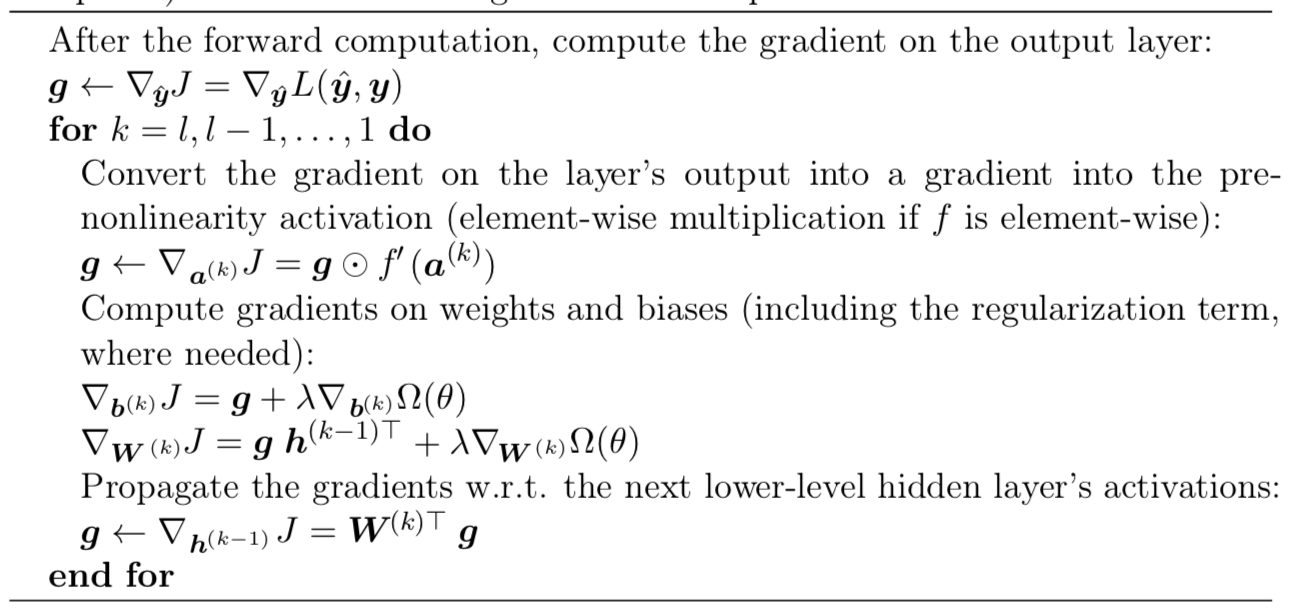
\includegraphics[width=0.6\textwidth]{note_images/backprop_algo.png} %插入图片,[]中设置图片大小,{}中是图片文件名
  \end{figure}

  
\end{document}
